\section{Estrategia utilizada}

\subsection{Descripción del \emph{Turtlebot}}

El robot utilizado en esta práctica es un \textit{Turtlebot} con lídar. Este escáner permite obtener un nube de puntos en 360º mapeándolos de la forma indicada en los ejes de la Figura \ref{fig:robot}.

\begin{figure}[!ht]
    \centering
    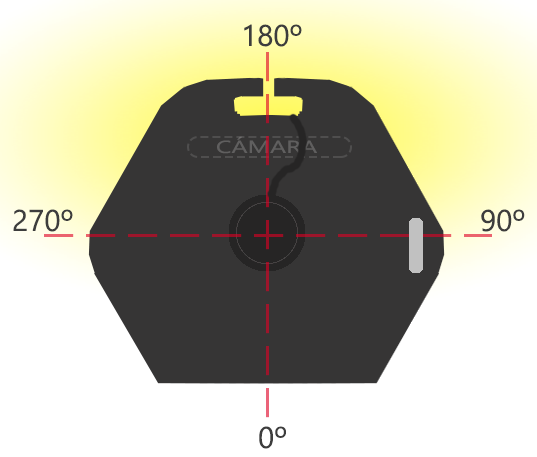
\includegraphics[scale=0.35]{images/robot.png}
    \caption{Esquema del robot \textit{Turtlebot}.}
    \label{fig:robot}
\end{figure}


\subsection{\emph{Topics} utilizados}
Para resolver esta práctica, la primera tarea es obtener la información del entorno. Nuestro robot \textit{Turtlebot} está provisto de un dispositivo lídar que permite obtener un nube de puntos en 360º, aunque en este caso sólo nos interesa utilizar los 180º que comprenden la parte delantera, como se indica en la Figura \ref{fig:robot}. Por tanto, utilizaremos la información recibida entre los 90º y los 270º. Esta nube de puntos la proporciona el \emph{topic} \texttt{scan} correspondiente al lídar, el cuál implementa el formato de mensaje \texttt{sensor\_msgs::LaserScan} con lo siguientes datos:


   \texttt{std\_msgs/Header header} 
\\ \tab \texttt{uint32 seq}
\\ \tab \texttt{time stamp} 

 \texttt{string frame\_id} 
 
 \texttt{float32 angle\_min} 
 
 \texttt{float32 angle\_max} 
 
 \texttt{float32 angle\_increment} 
 
 \texttt{float32 time\_increment} 
 
 \texttt{float32 scan\_time} 
 
 \texttt{float32 range\_min} 
 
 \texttt{float32 range\_max} 
 
 \texttt{float32[] ranges} 
 
 \texttt{float32[] intensities} 


Como vemos, el escáner proporciona gran cantidad de información, aunque los datos que realmente nos van a ser útiles en esta tarea se encuentran en el array \texttt{float32[] ranges}, que indica la distancia a la que se encuentra cada punto detectado para cada uno de los ángulos. De esta manera, la suscripción a este \emph{topic} nos permite conocer la situación del robot con el entorno prácticamente en tiempo real. 

Desde el \textit{topic} de odometría obtenemos la siguiente información del mensaje \texttt{nav\_msgs/Odometry}:
 
 \texttt{Header header}
 
 \texttt{string child\_frame\_id}
 
\texttt{geometry\_msgs/PoseWithCovariance pose}
 
 \texttt{geometry\_msgs/TwistWithCovariance twist}
 
Utilizaremos la información de \texttt{pose} para conocer la posición y la rotación del robot.

Por último, en este caso, para aplicar la velocidad de movimiento al robot, se utiliza el modulo \textit{teleop} previamente implementado.


\subsection{Mapeado del entorno}

Gracias a la odometría podemos conocer en cada momento las posiciones $x_r$ e $y_r$ del robot, así como su ángulo de orientación $\theta_r$.

Además, para cada uno de los 180 puntos detectados por el láser, tenemos la información de la distancia $I$ a la que se ha detectado y el ángulo $\theta_l$ al que corresponde.

Hemos establecido un umbral de 5 metros para dibujar sólo aquellos puntos que se detecten por debajo de esa distancia y así, con esta información es posible proyectar cada punto detectado en el mapa.

\[x_m = x_r + I*cos(\theta_r + \theta_l)\]
\[y_m = y_r + I*sin(\theta_r + \theta_l)\]

De esta manera, para cada instante de tiempo obtenemos las coordenadas de cada punto $x_m, y_m$ a dibujar en el mapa, como se muestra en la Figura \ref{fig:map_pasillo}.

\begin{figure}[!ht]
\centering
    \subfigure[]{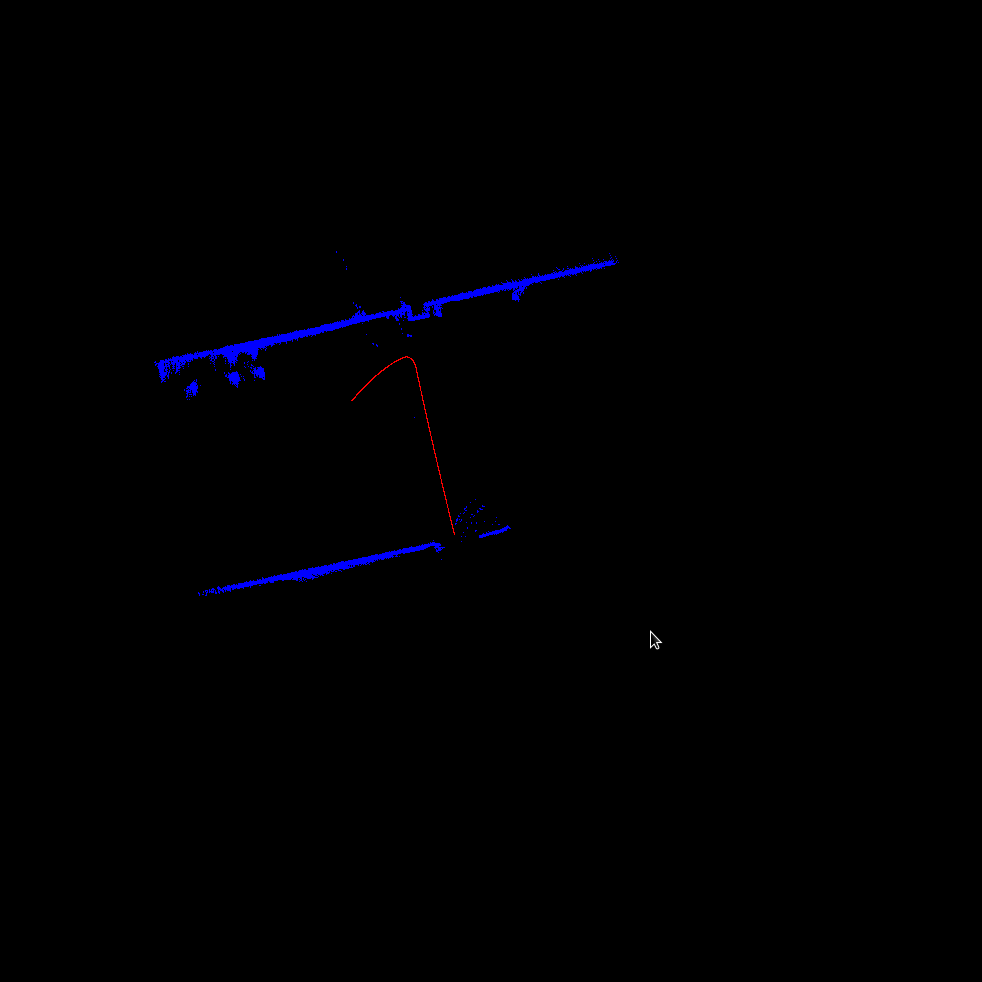
\includegraphics[width=45mm]{images/1.png}}
    \subfigure[]{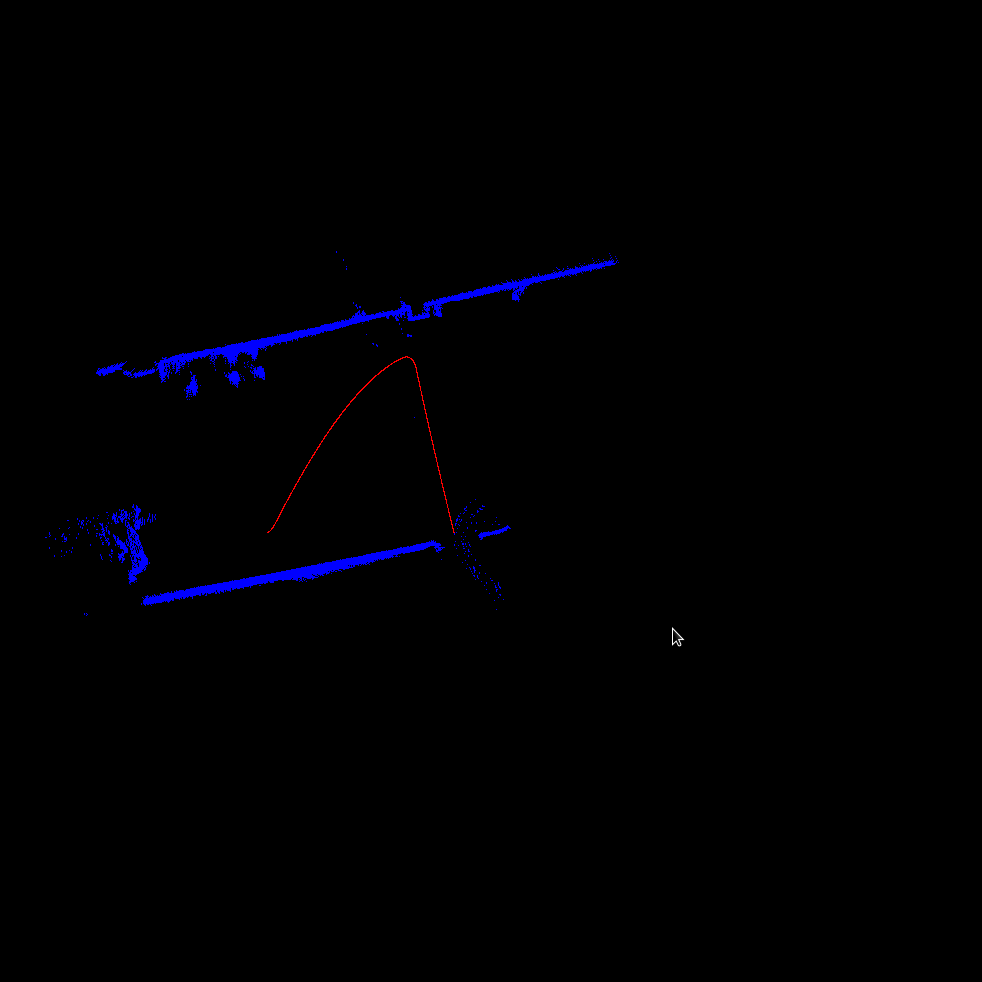
\includegraphics[width=45mm]{images/3.png}}
    \subfigure[]{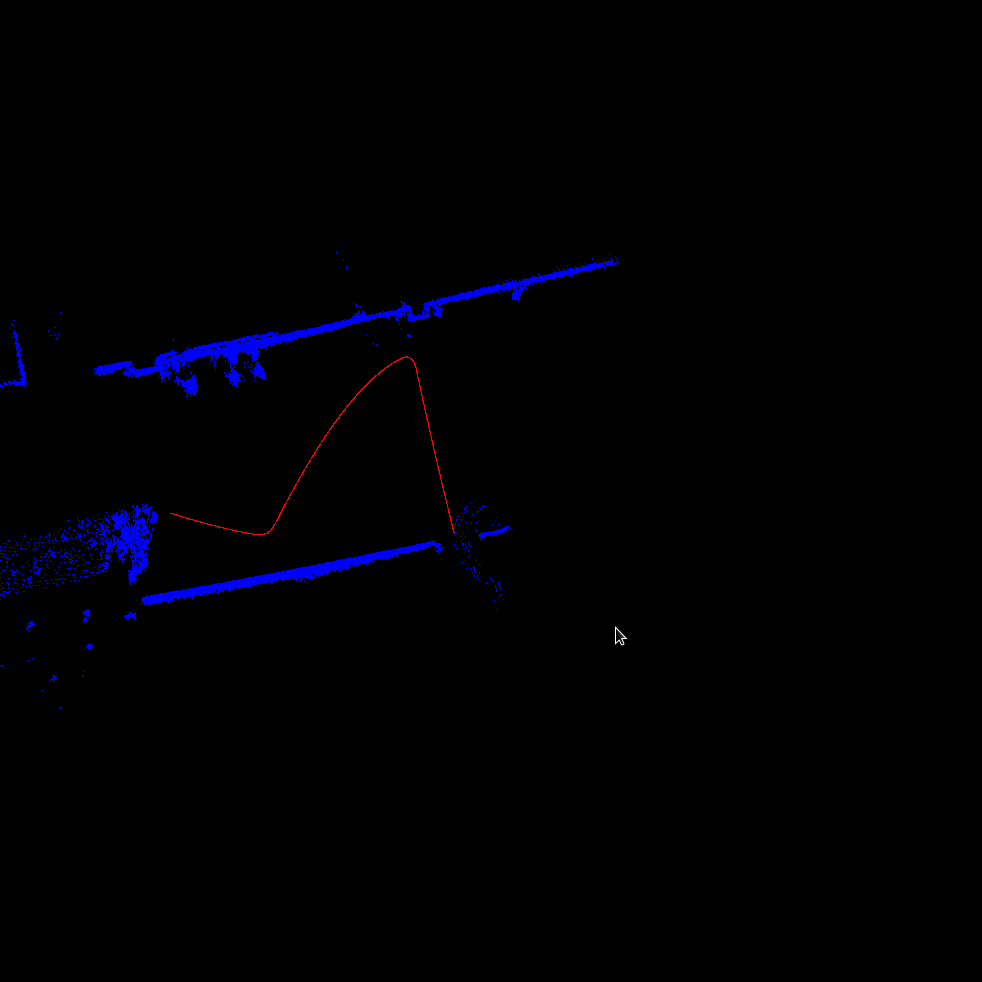
\includegraphics[width=45mm]{images/4.png}}
    \caption{Construcción progresiva del mapa del pasillo. A la izquierda de cada imagen, se encontrarían la escaleras, a la derecha, el laboratorio de los otros compañeros y en el punto de partida, la salida de nuestro laboratorio.} \label{fig:map_pasillo}
\end{figure}

